%%%%%%%%%%%%%%%%%%%%%%%%%%%%%%%%%%%%%%%%%%
% Github: github.com/Amir1453
%
%
%Eğer fotoğraf eklemek istiyorsanız ./images klasörüne atın.
% 
%Kapak sayfasını başka bir yerde yapıp ilk sayfayı kaldırıp
%pdfleri birleştirebilirsiniz.
%
%
%%%%%%%%%%%%%%%%%%%%%%%%%%%%%%%%%%%%%%%%%

%_--------------------------------------
% 
% FOTOĞRAF EKLERKEN BÖYLE EKLMENİZ LAZIM ÇÜNKÜ BABEL TÜRKÇE İLE ALAKALI BİR BUG VAR!
%
%\shorthandoff{=}
%\begin{figure}[H]
%    \centering
%    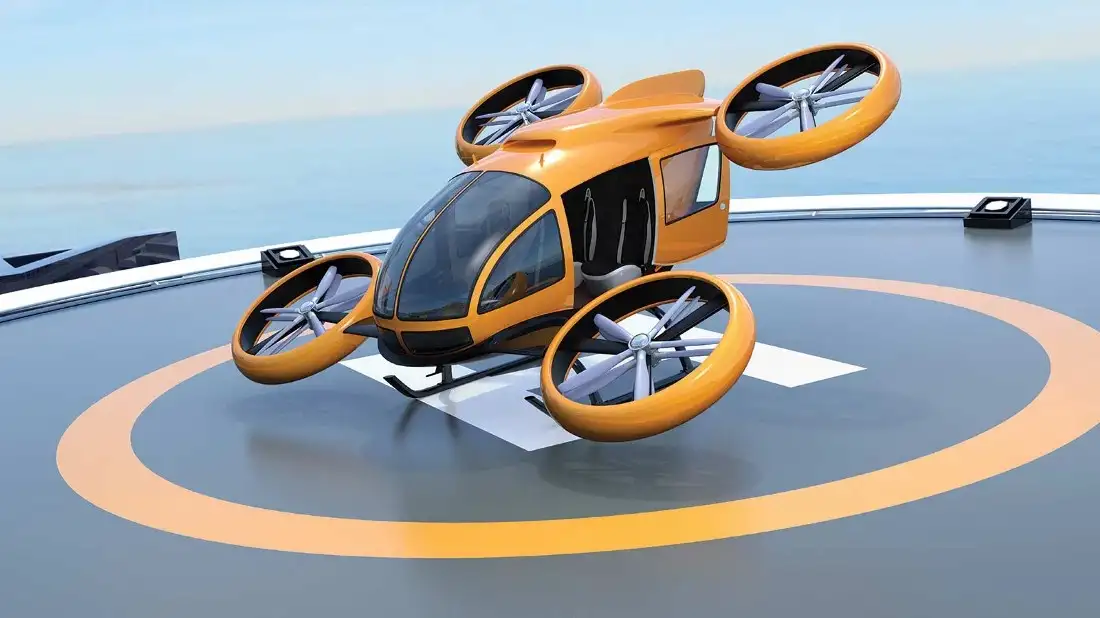
\includegraphics[scale=0.40]{images/flyingcar.png}
%    \caption{Caption}
%    \label{fig:my_label}
%\end{figure}
%\shorthandon{=}
%-------------------------------------------
%
% REFERANS YAPMAK İÇİN \cite{} KULLANIN. 
%bibliography.bib DOSYASINA BIBTEX FORMATINDA 
%REFERANSLARINIZI KOYABILIRINSIZ.
%DAHA ÇOK BİLGİ İÇİN LÜTFEN ARAŞTIRIN.
%https://www.overleaf.com/learn/latex/Bibliography_management_with_bibtex
%-----------------------------------------
%Section, subsection, subsubsection paragraph 
%şeklinde alt başlıklara ayırabilirsiniz.
%table of contents otomatik olarak içindekiler yapacktır.
%İstediğiniz gibi değiştirebilirsiniz, size kalmış.
%-------------------------------------------




%establishing document class with 12pt
\documentclass[12pt]{article}



\usepackage[turkish]{babel} %Türkçe bölüm isimleri
\usepackage[utf8]{inputenc} %Türkçe karakterler
\usepackage[T1]{fontenc} %Türkçe heceleme

%Packages used for the background image

\usepackage{xcolor}
\usepackage{graphicx}
\graphicspath{./images}
\usepackage{float}
\usepackage{eso-pic}
\usepackage[export]{adjustbox}

%Package used for making hyperlinks
\usepackage[hidelinks]{hyperref}

%Times New Roman
\usepackage{times}

% for reference urls to work.
\usepackage{url}

%Package for bibliography
\usepackage[sorting=none,backend=bibtex]{biblatex}
\addbibresource{bibliography.bib}

%Adding TEKNOFEST watermark
\newcommand\BackgroundPicture{
   \put(0,0){
     \parbox[b][\paperheight]{\paperwidth}{
       \vfill
		%\node[opacity=0.69]
       \centering
\includegraphics[width=0.7\paperwidth,height=0.7\paperheight,keepaspectratio]{background.png}
       \vfill
     }}}
\AddToShipoutPicture{\BackgroundPicture}
%----------------------------------


% TEKNOFESTin istediği formata uygun yapmak için
% sayfa sayısı ve sayfanın altına takım ismi
\usepackage{fancyhdr}
\pagestyle{fancy}
\renewcommand{\headrulewidth}{0pt}
\fancyhf{}
\fancyhead[R]{\thepage}
%TAKIM ISMINIZI GIRIN
\fancyfoot[C]{TAKIM ADI}



%Begin the document
\begin{document}

\begin{center}
    \Huge BLANK PAGE    
\end{center}

%ilk sayfayı boş bırakıyor.
\newpage

%Creating a table of contents
\tableofcontents

\newpage




\section{Senaryo ve Hava Trafik Yöntemi}



\subsection{Genel Trafik Modeli}
%BURAYA YAZI GELECEK

\subsection{Hava Araçlarının Hareket Kuralları}

\subsubsection{Araçların kurallara uyabilmesi için gereken özellikler}
%BURAYA YAZI GELECEK
\subsubsection{Kullanıcıların Yükümlülükleri}
%BURAYA YAZI GELECEK
\subsubsection{Kurallara uyulmaması durumunda yaptırımlar}
%BURAYA YAZI GELECEK
\subsubsection{Hava araçlarının tam otonom olma süreci}
%BURAYA YAZI GELECEK

\subsection{Hava Araçlarında Komünikasyon}

\subsubsection{Araçlar arası komünikasyon}
%BURAYA YAZI GELECEK
\subsubsection{Araçlar ve merkez arası komünikasyon}
%BURAYA YAZI GELECEK
\subsubsection{Araçlar ve kalkış iniş noktaları arası komünikasyon}
%BURAYA YAZI GELECEK

\subsection{Araca Biniş ve İniş}

\subsubsection{Merkezi duraklar}
%BURAYA YAZI GELECEK
\subsubsection{Bireysel kullanım}
%BURAYA YAZI GELECEK

\subsection{Rota Planlama}

\subsubsection{Varış noktası seçimi}
%BURAYA YAZI GELECEK
\subsubsection{Seyahat sırasında daha optimal rota tespiti}
%BURAYA YAZI GELECEK
\subsubsection{Kullanıcı tarafından varış noktasının değiştirilmesi}
%BURAYA YAZI GELECEK
\subsubsection{Şehir içi ve dışı rotalar}
%BURAYA YAZI GELECEK

\subsection{İdeal Olmayan Durumlara Karşı Tepki}

\subsubsection{Değişken hava durumu}
%BURAYA YAZI GELECEK
\subsubsection{Beklenmedik trafik yoğunluğu}
%BURAYA YAZI GELECEK
\subsubsection{Acil durumlar}
%BURAYA YAZI GELECEK

\subsection{Yakıt/Batarya}

\subsubsection{Batarya/yakıt kapasitesinin yönetimi}
%BURAYA YAZI GELECEK
\subsubsection{Şarj/dolumun hangi aralıklarla yapılacağı}
%BURAYA YAZI GELECEK
\subsubsection{Şarj/dolumun nerede yapılacağı}
%BURAYA YAZI GELECEK

% Yeni sayfa ve referansları yazdırıyor.

\newpage
% Eğer refernsa eklemek istediğiniz ama citelamadığınız bir şey olursa buraya yazın.
%\nocite{citekey}
\printbibliography
    
\end{document}
